%%%%%%%%%%%%%%%%%%%%%%%%%%%%%%%%%%%%%%%%%
% University/School Laboratory Report
% LaTeX Template
% Version 3.1 (25/3/14)
%
% This template has been downloaded from:
% http://www.LaTeXTemplates.com
%
% Original author:
% Linux and Unix Users Group at Virginia Tech Wiki 
% (https://vtluug.org/wiki/Example_LaTeX_chem_lab_report)
%
% License:
% CC BY-NC-SA 3.0 (http://creativecommons.org/licenses/by-nc-sa/3.0/)
%
%%%%%%%%%%%%%%%%%%%%%%%%%%%%%%%%%%%%%%%%%

%----------------------------------------------------------------------------------------
%	PACKAGES AND DOCUMENT CONFIGURATIONS
%----------------------------------------------------------------------------------------

\documentclass{article}

\usepackage{graphicx} % Required for the inclusion of images
\usepackage{natbib} % Required to change bibliography style to APA
\usepackage{amsmath} % Required for some math elements
\usepackage{mathtools}
\usepackage[export]{adjustbox}
\usepackage{subcaption}
\usepackage{float}
\usepackage{listings}
\usepackage{minted}

\DeclarePairedDelimiter{\abs}{\lvert}{\rvert}
\setlength\parindent{0pt} % Removes all indentation from paragraphs

\renewcommand{\labelenumi}{\alph{enumi}.} % Make numbering in the enumerate environment by letter rather than number (e.g. section 6)

%\usepackage{times} % Uncomment to use the Times New Roman font

%----------------------------------------------------------------------------------------
%	DOCUMENT INFORMATION
%----------------------------------------------------------------------------------------

\title{ECE 637 Digital Image Filtering Laboratory: \\ Image Filtering} % Title

\author{Yang \textsc{Wang}} % Author name

\date{\today} % Date for the report

\begin{document}

\maketitle % Insert the title, author and date

% If you wish to include an abstract, uncomment the lines below
% \begin{abstract}
% Abstract text
% \end{abstract}

%----------------------------------------------------------------------------------------
%	SECTION 1
%----------------------------------------------------------------------------------------

\section{C Programming}

Nothing due for report.

% If you have more than one objective, uncomment the below:
%\begin{description}
%\item[First Objective] \hfill \\
%Objective 1 text
%\item[Second Objective] \hfill \\
%Objective 2 text
%\end{description}

%\subsection{Definitions}
%\label{definitions}
%\begin{description}
%\item[Stoichiometry]
%The relationship between the relative quantities of substances taking part in a reaction or forming a compound, typically a ratio of whole integers.
%\item[Atomic mass]
%The mass of an atom of a chemical element expressed in atomic mass units. It is approximately equivalent to the number of protons and neutrons in the atom (the mass number) or to the average number allowing for the relative abundances of different isotopes. 
%\end{description} 
 
%----------------------------------------------------------------------------------------
%	SECTION 2
%----------------------------------------------------------------------------------------

\section{Displaying and Exporting Images in Matlab}

Nothing due for report.

%----------------------------------------------------------------------------------------
%	SECTION 3
%----------------------------------------------------------------------------------------

\section{FIR Low Pass Filter}

In this section, an supplied image is filtered with a 9 $\times$ 9 low pass filter given as:
\begin{equation}
\textit{h}(\textit{m},\textit{n}) = \begin{cases}1/81 & \text{for } \abs{m} \le 4 \text{, } \abs{n} \le 4\\
0 & \text{otherwise}\\
\end{cases}
\end{equation}

\subsection{Find DSFT of FIR low pass filter}
\begin{description}
\item[]
Using DSFT formula, we have:
\begin{align*}
H(e^{j\mu},e^{j\nu}) &= {\sum_{n=-4}^{4}\sum_{m=-4}^{4}}\frac{1}{81}e^{-j(m\mu+n\nu)} \\
					 &= \frac{1}{81}{\sum_{n=-4}^{4}}e^{-jm\mu}{\sum_{n=-4}^{4}}e^{-jm\nu}
\end{align*}
We know the formula:
\begin{equation}
{\sum_{n=-N}^{N}}e^{-j\omega n} = e^{j\omega N}\frac{1-e^{-j\omega (2N+1)}}{1-e^{-j\omega}}
\end{equation}
Therefore,
\begin{align*}
H(e^{j\mu},e^{j\nu}) &= \frac{1}{81}{{\sum_{n=-4}^{4}}\frac{e^{j4\mu}-e^{-j5\mu}}{1-e^{-j\mu}}}
{{\sum_{n=-4}^{4}}\frac{e^{j4\nu}-e^{-j5\nu}}{1-e^{-j\nu}}} \\
					 &= \frac{1}{81}{\frac{sin(\frac{9}{2}\mu)}{sin(\frac{1}{2}\mu)}}
                     {\frac{sin(\frac{9}{2}\nu)}{sin(\frac{1}{2}\nu)}}
\end{align*}
\end{description}

\subsection{Plot the magnitude of DSFT of FIR low pass filter}
\begin{figure}[h]
\begin{center}
\includegraphics[width=0.8\textwidth]{lpfcsft}
\caption{Magnitude of LPF.}
\end{center}
\end{figure}

\subsection{Original vs. filtered image}
The images from the next page shows that the filtered image is more blurred out than the original image as it goes through the low pass filter.
\pagebreak
\begin{figure}[h]
\begin{subfigure}{0.5\textwidth}
\includegraphics[width=0.9\linewidth, left]{img03} 
\caption{img03.tif}
\end{subfigure}
\begin{subfigure}{0.5\textwidth}
\includegraphics[width=0.9\linewidth, right]{firlpf}
\caption{lpfimg03.tif}
\end{subfigure}
\caption{Original vs. Low-Pass Filtered Image}
\end{figure}

\subsection{Code listing}
\subsubsection{firlpf.c}
This listing loads, manipulates the image with a 2-D convolution, and writes to a new image.
\inputminted[tabsize=4]{c}{firlpf.c}
\subsubsection{defs.c}
This listing specifies C implementation for 2-D convolution, and other helper functions.
\inputminted[tabsize=4]{c}{defs.c}
\subsubsection{defs.h}
\inputminted[tabsize=4]{c}{defs.h}

%----------------------------------------------------------------------------------------
%	SECTION 4
%----------------------------------------------------------------------------------------

\section{FIR Sharpening Filter}

In this section, the effect of a FIR sharpening filter on an image is analyzed. An supplied image is filtered with a FIR sharpening filter H(m,n) which is constructed using a 5 $\times$ 5 FIR low pass filter given as:
\begin{equation}
\textit{h}(\textit{m},\textit{n}) = \begin{cases}1/25 & \text{for } \abs{m} \le 2 \text{, } \abs{n} \le 2 \\
0 & \text{otherwise}\\
\end{cases}
\end{equation}
and,
\begin{equation}
\textit{g}(\textit{m},\textit{n}) = \delta(\textit{m},\textit{n})+\lambda(\delta(\textit{m},\textit{n})-\textit{h}(\textit{m},\textit{n}))
\end{equation}

\subsection{Find an expression for FIR low pass filter}
\begin{description}
\item[]
Using the same method as in Section 3, we have:
\begin{align*}
H(e^{j\mu},e^{j\nu}) &= {\sum_{n=-2}^{2}\sum_{m=-2}^{2}}\frac{1}{25}e^{-j(m\mu+n\nu)} \\
					 &= \frac{1}{25}{\sum_{n=-2}^{2}}e^{-jm\mu}{\sum_{n=-2}^{2}}e^{-jm\nu}
\end{align*}
Using equation (2):
\begin{align*}
H(e^{j\mu},e^{j\nu}) &= \frac{1}{25}{{\sum_{n=-2}^{2}}\frac{e^{j2\mu}-e^{-j3\mu}}{1-e^{-j\mu}}}
{{\sum_{n=-2}^{2}}\frac{e^{j2\nu}-e^{-j3\nu}}{1-e^{-j\nu}}} \\
					 &= \frac{1}{25}{\frac{sin(\frac{5}{2}\mu)}{sin(\frac{1}{2}\mu)}}
                     {\frac{sin(\frac{5}{2}\nu)}{sin(\frac{1}{2}\nu)}}
\end{align*}
\end{description}

\subsection{Find an expression for FIR sharpening filter}
\begin{description}
\item[]
Using the result in Section 4.2, we have:
\begin{align*}
G(e^{j\mu},e^{j\nu}) &= 1+\lambda(1-H(e^{j\mu},e^{j\nu})) \\
					 &= 1+\lambda(1-\frac{1}{25}{\frac{sin(\frac{5}{2}\mu)}{sin(\frac{1}{2}\mu)}}
                     {\frac{sin(\frac{5}{2}\nu)}{sin(\frac{1}{2}\nu)}})
\end{align*}
\end{description}
\pagebreak

\subsection{Plot the magnitude of LPF}
\begin{figure}[h]
\begin{center}
\includegraphics[width=0.6\textwidth]{lpf1csft}
\caption{Magnitude of LPF.}
\end{center}
\end{figure}

\subsection{Plot the magnitude of HPF}
\begin{figure}[h]
\begin{center}
\includegraphics[width=0.6\textwidth]{hpfcsft}
\caption{Magnitude of HPF for $\lambda$=1.5.}
\end{center}
\end{figure}

\subsection{Original vs. filtered image}
The images from the next page show that the filtered image is more sharpened than the original image as it goes through the high pass filter.
\begin{figure}[h]
\begin{subfigure}{0.5\textwidth}
\includegraphics[width=0.9\linewidth, left]{imgblur} 
\caption{imgblur.tif}
\end{subfigure}
\begin{subfigure}{0.5\textwidth}
\includegraphics[width=0.9\linewidth, right]{firsf}
\caption{sfimg03.tif}
\end{subfigure}
\caption{Original vs. High-Pass Filtered Image ($\lambda$=1.5).}
\end{figure}

\subsection{Code listing}
\subsubsection{firsf.c}
This code loads, manipulates an image with a sharpening filter, and writes to a new image.
\inputminted[tabsize=4]{c}{firsf.c}
\subsubsection{defs.c}
This listing uses the same code in Section 3.4.2.
\subsubsection{defs.h}
This listing uses the same code in Section 3.4.3.

%----------------------------------------------------------------------------------------
%	SECTION 5
%----------------------------------------------------------------------------------------

\section{IIR Filter}

In this section, the effect of an IIR filter specified by a 2-D difference equation is analyzed. The 2-D equation is given as the following:
\begin{equation}
y(m,n)=0.01x(m,n)+0.9(y(m-1,n)+y(m,n-1))-0.81(y(m-1,n-1))
\end{equation}

\subsection{Find an expression for IIR}
\begin{description}
\item[]
Taking the Z-transform of both sides on equation (5):
\begin{align*}
Y(z_1,z_2) &= 0.01X(z_1,z_2)+0.9z_1^{-1}Y(z_1,z_2)+0.9z_2^{-1}Y(z_1,z_2)-0.81z_1^{-1}z_2^{-1}Y(z_1,z_2) \\
0.01X(z_1,z_2) &= Y(z_1,z_2)-0.9z_1^{-1}Y(z_1,z_2)-0.9z_2^{-1}Y(z_1,z_2)
\end{align*}
\begin{equation}
\frac{Y(z_1,z_2)}{X(z_1,z_2)} = H(z_1,z_2) = \frac{0.01}{1-0.9z_1^{-1}-0.9z_2^{-1}+0.81z_1^{-1}z_2^{-1}}
\end{equation}
We have the relations:
\begin{align*}
z_1 &= e^{j\mu} \\
z_2 &= e^{j\nu}
\end{align*}
Substituting into equation (6):
\begin{equation}
H(e^{j\mu},e^{j\nu}) = \frac{0.01}{1-0.9e^{-j\mu}-0.9e^{-j\nu}+0.81e^{-j(\mu + \nu)}}
\end{equation}
\end{description}

\subsection{Plot the magnitude of IIR Filter}
\begin{figure}[h]
\begin{center}
\includegraphics[width=0.8\textwidth]{iircsft}
\caption{Magnitude of IIR Filter.}
\end{center}
\end{figure}

\pagebreak

\subsection{Image of the point spread function}
\begin{figure}[h]
\begin{center}
\includegraphics[width=0.8\textwidth]{hout}
\caption{255 $\times$ 100 Image of Point Spread Function.}
\end{center}
\end{figure}

\subsection{Original vs. filtered image}
The images on the next page show that the filtered image is "smeared out". This is due to that the difference equation is trying to average out the value by taking past output values in the sum.

\pagebreak

\begin{figure}[ht]
\begin{subfigure}{0.5\textwidth}
\includegraphics[width=0.9\linewidth, left]{img12} 
\caption{img12.tif} 
\end{subfigure}
\begin{subfigure}{0.5\textwidth}
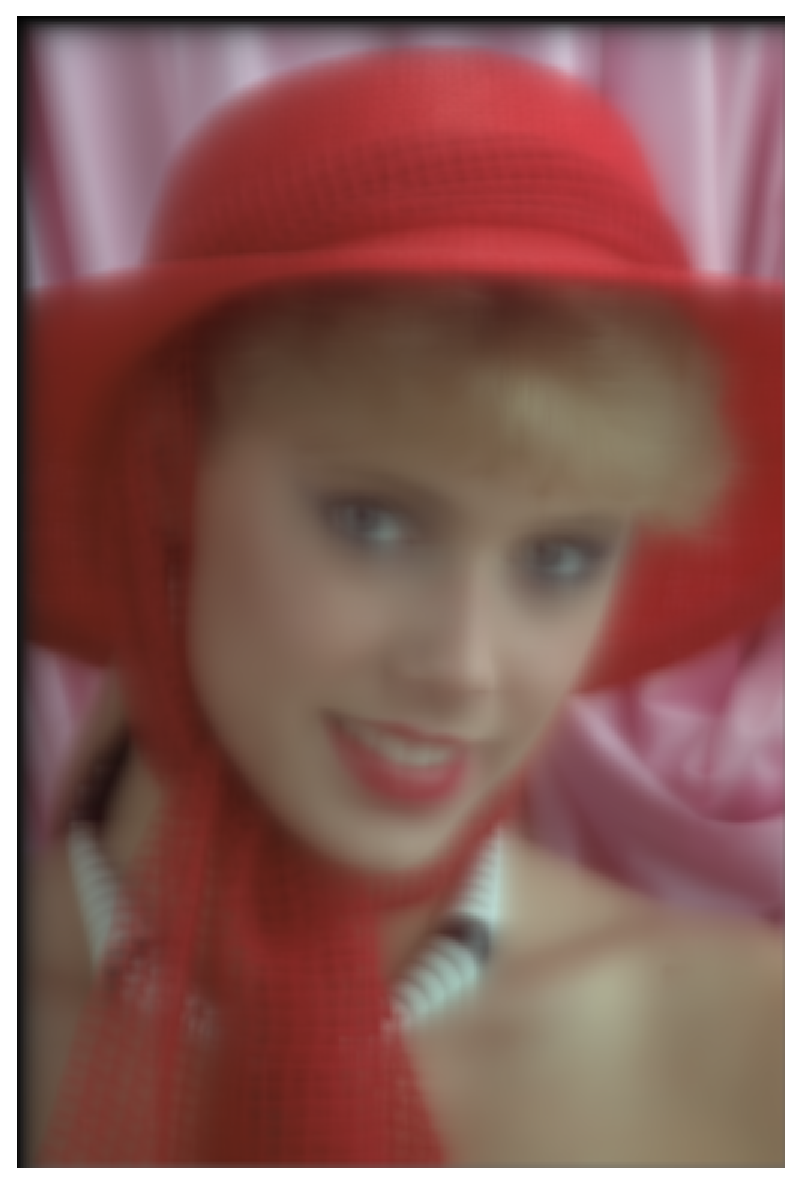
\includegraphics[width=0.9\linewidth, right]{iirf}
\caption{iirfimg12.tif}
\end{subfigure}
\caption{Original vs. IIR Filtered Image}
\end{figure}

\subsection{Code listing}
\subsubsection{iirf.c}

\inputminted[tabsize=4]{c}{iirf.c}
\subsubsection{defs.c}
This listing uses the same code in Section 3.4.2.
\subsubsection{defs.h}
This listing uses the same code in Section 3.4.3.

\end{document}
